% Keep the overview and the combined acceptance/rate figure consecutive.
\clearpage
\begin{figure}[p]
\centering
\begin{minipage}[t]{0.48\linewidth}
\centering\small\textbf{Aligned geometry used for the rates}\par\medskip
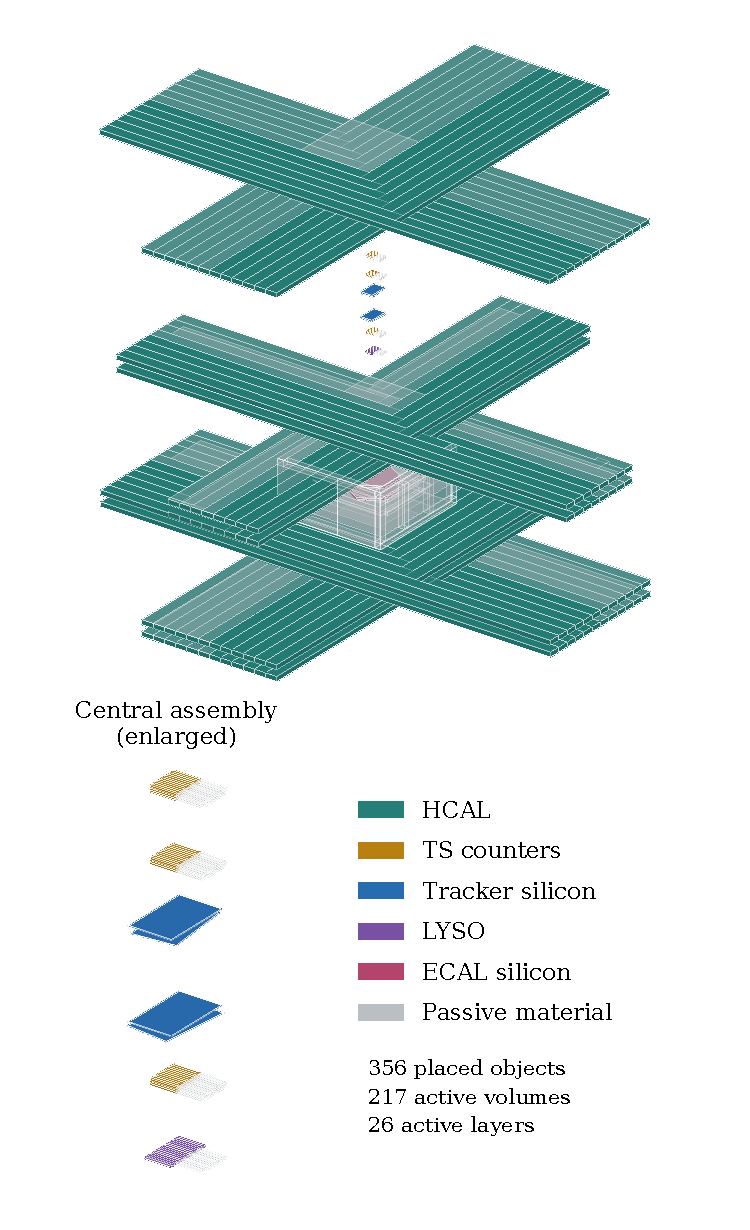
\includegraphics[width=\linewidth]{combinations_20260919/figures/full_installed_geometry.pdf}
\end{minipage}\hfill
\begin{minipage}[t]{0.49\linewidth}
\centering\small\textbf{Earlier offset layout: accepted rays}\par\medskip
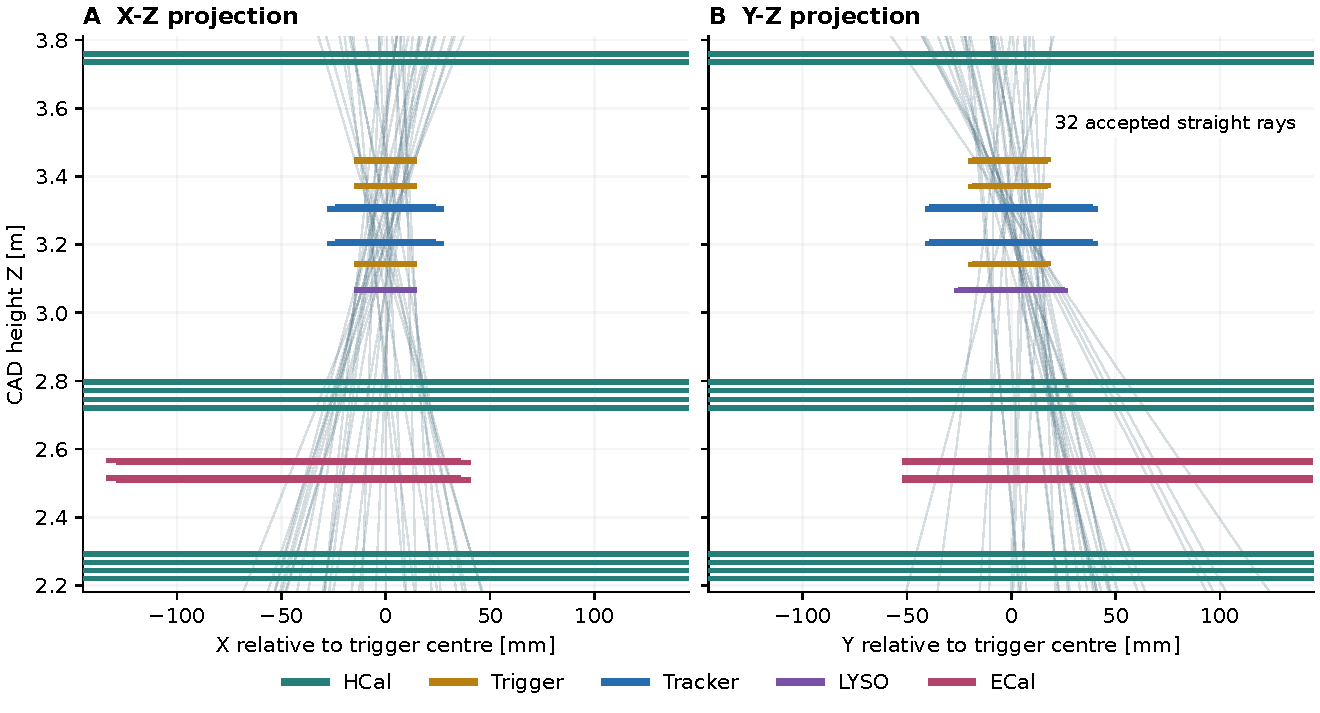
\includegraphics[height=2.88in,trim=0 26 300 0,clip]{geometry_acceptance.pdf}\par\medskip
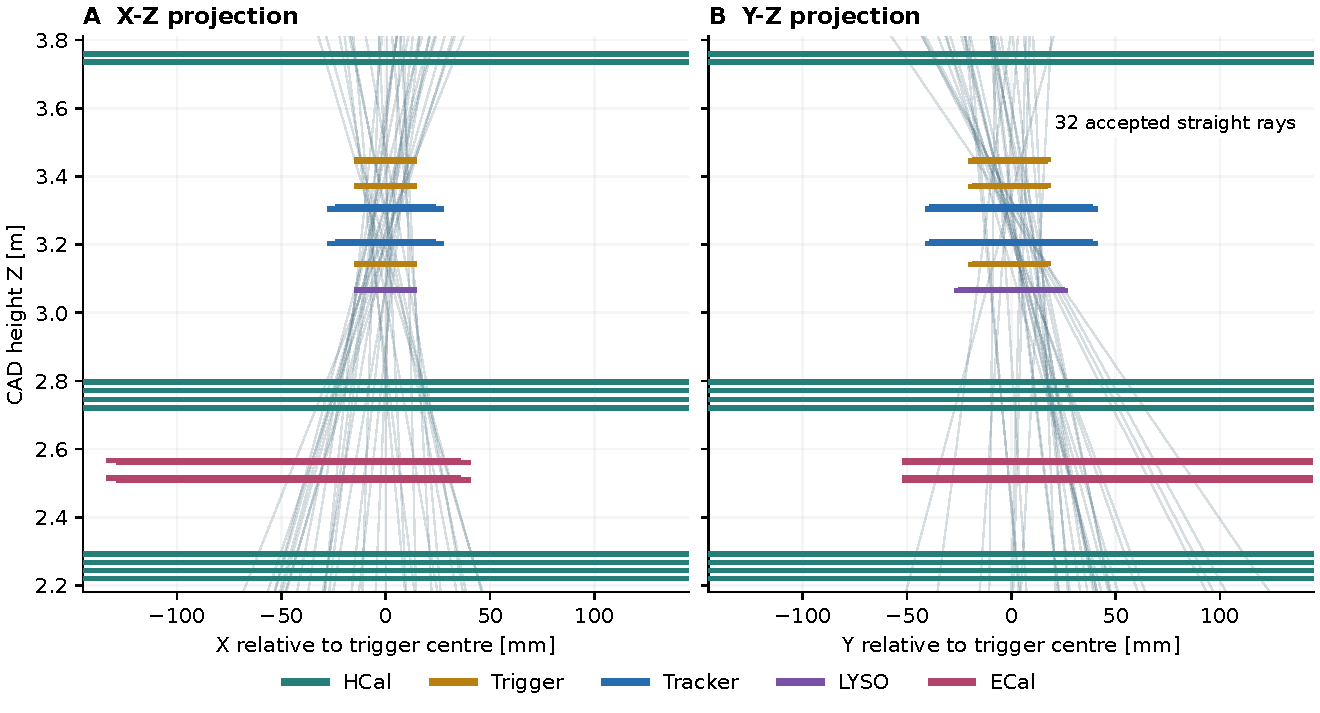
\includegraphics[height=2.88in,trim=336 26 0 0,clip]{geometry_acceptance.pdf}
\end{minipage}
\caption{\textbf{Installed geometry and the accepted-ray aperture.}
Left: the complete aligned detector model, with passive material shown
translucently and a separate enlargement of the central assembly below.
CAD stand supports are outside the material model. Right: the previous rate
report's 32 accepted straight rays, with its original vector projections
stacked for readability. These rays use the earlier \emph{offset} ECAL;
all main-table rates use the aligned layout. Colours identify the same
subsystems in both panels. The rays include no scattering or detector response.}
\label{fig:overview}
\end{figure}
\clearpage
\begin{figure}[p]
\centering
{\small\textbf{(a) Active-layer envelopes in the aligned layout}}\par\smallskip
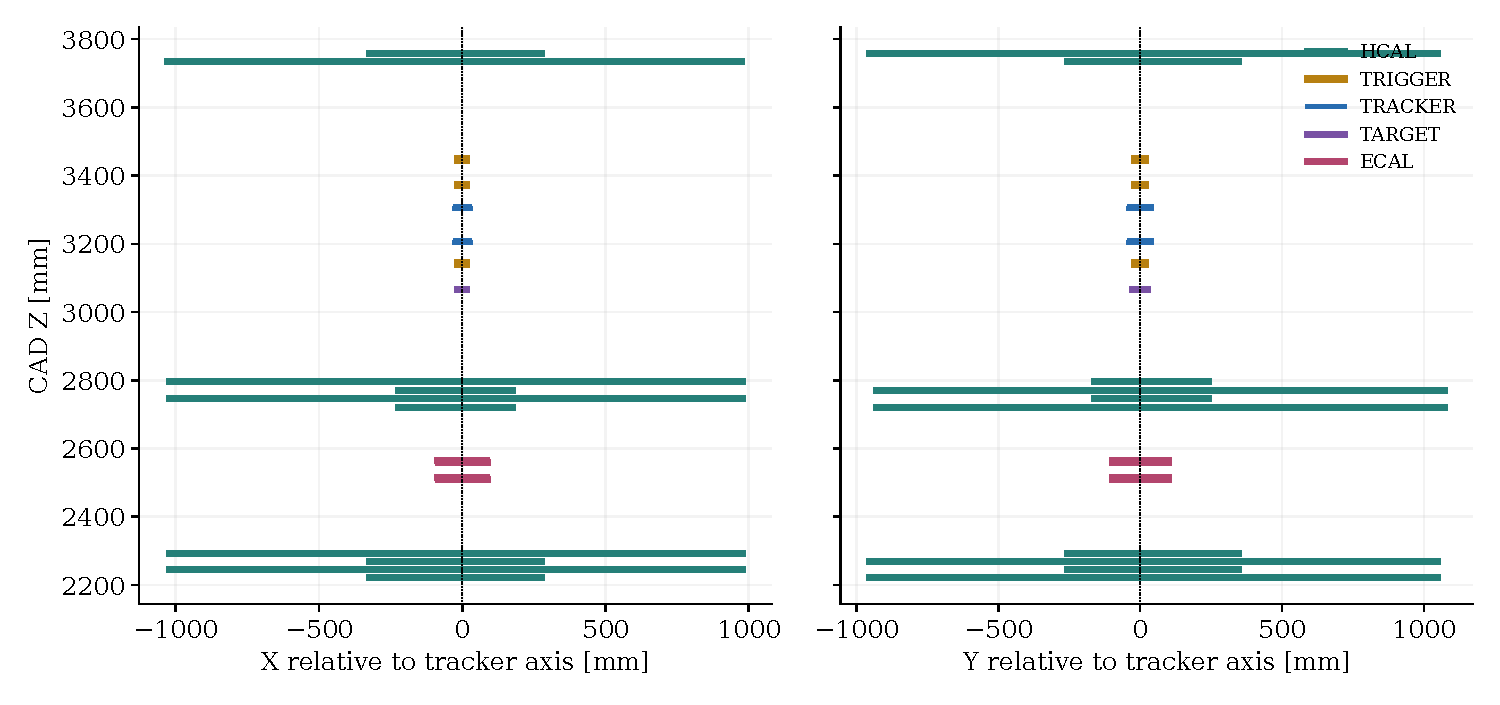
\includegraphics[width=0.98\linewidth]{combinations_20260919/figures/aligned_geometry.pdf}\par\medskip
{\small\textbf{(b) Rates retained by representative detector requirements}}\par\smallskip
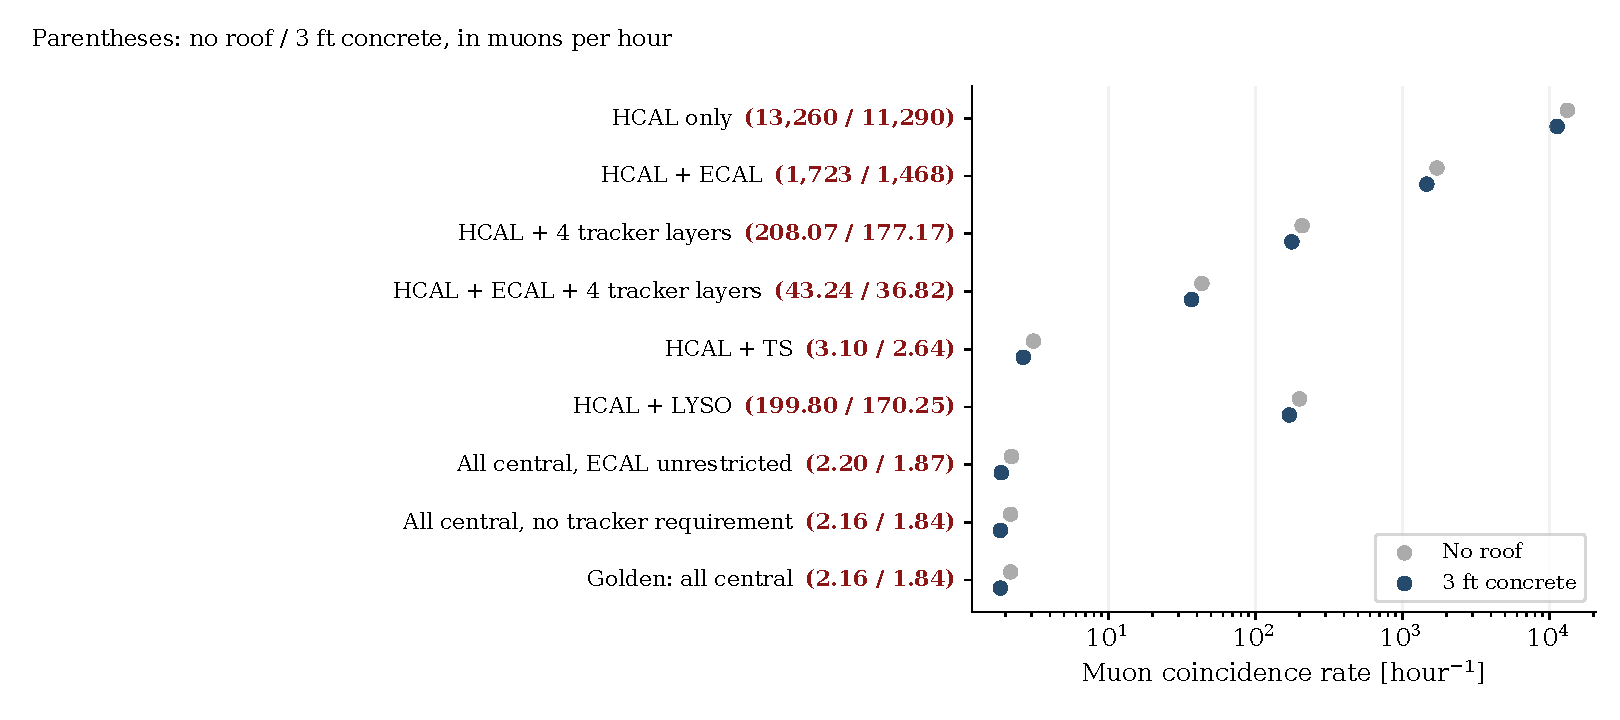
\includegraphics[width=0.98\linewidth]{combinations_20260919/figures/rate_hierarchy.pdf}
\caption{\textbf{From detector aperture to coincidence rate.}
(a) The active-layer envelopes, with transverse coordinates measured from
the tracker axis and heights in CAD $Z$. Line thicknesses are enlarged for
visibility; the calculation retains the segmented solids.
(b) Inclusive selections requiring all ten HCAL layers, on a logarithmic rate
axis. ``All central'' requires all TS, LYSO, ECAL and tracker layers.
``ECAL unrestricted'' keeps ECAL installed but imposes no ECAL hit requirement:
events may hit or miss it, while all other listed hit requirements still apply.
``No tracker requirement'' similarly leaves tracker hits unrestricted. The same aligned
geometry and sea-level spectrum are used for both roof assumptions. Bold red
values beside each selection give the rate per hour (no roof / 3 ft concrete).}
\label{fig:summary}
\label{fig:geometry}
\label{fig:hierarchy}
\end{figure}
\clearpage
